\chapter{Evaluation}
%%\textbf{In an ideal world, you should have two kind of evaluations.  The first is against some ground truth (perhaps a random model?).  The second kind of evaluation is against other people's work (accuracy, speed, etc.).  Any dimension which is of interest, should be evaluated.  Evaluation should be statistically sound. }
In this chapter, we interpret our experiment results against a backdrop of reviewed literature.  We divided our experiments in two parts.  In the first instance, we compared the reviewed projection learning techniques by evaluating them on a common dataset and evaluation metrics platform.  Each algorithm features specialised hyperparameters which - according to the original literature - were reported to have some influence on performance.  We built two out of the three algorithms from first principles, following the technical instructions in the respective papers \citep{ustalov2017negative, bernier2018crim}.  

We leveraged the \ac{ANOVA} framework to confirm or reject the hypothesis that a feature has an effect on score.  Before quoting the test's $F-$score and related $p-$value, we confirm that the three conditions for \ac{ANOVA} are met: normal distribution of the data points; homogeneity of variance; independent observations.  We use Jarque-Bera to test for normality; Omnibus to test for variance homogeneity; Condition Number to test for multicollinearity.  Whenever \ac{ANOVA} recommended that we reject the null hypothesis that the group means are equal, we ran Tukey \ac{HSD} post-hoc analysis which computes a series of pair-wise tests among the levels of a particular group to find out which factor levels have a significant effect on the model score.  We assume 95\% confidence throughout, which means we take a 5\% risk of committing a Type 1 error.

In the second set of experiments, we focused on our implementation of CRIM \citep{bernier2018crim} and applied the algorithm on SemEval-2018, Task 9 \citep{camacho2018semeval}.  We motivated our decision by our experience in the previous set of experiments, where we found CRIM to perform well, was receptive to different embeddings and other settings, and was easy to train.  Moreover, it was the algorithm which yielded the highest scores in the English language tasks it was set out to solve in the actual shared task.  However, we apply a number of changes which enables us to reduce training epochs significantly (from an original range between 200 and 1000 to less than 20), particularly thanks to a simple transfer learning strategy we employ which lets us learn the projection matrices and tune the embeddings in two separate phases.

\section{Analyses of Projection Learning Models}
We split the evaluation in two, starting from an analysis of regularisation and cluster count on projection-learning algorithms which are training by minimising \ac{MSE}.  We, also explore the effect of embeddings, an analysis which hitherto has not been carried out by the research community.  In the second subsection, we focus on CRIM and Yamane, the models which leverage the dot-product to estimate the similarity between the predicted and actual hypernym, and which are trained to minimise the binary cross-entropy objective function.

\subsection{MSE Hard-Clustering Models}
We evaluate our results on the basis of five metrics, but we focus exclusively on \ac{MRR} and \ac{MAP} which provide two interesting facets of our discovered hypernyms: how highly the models ranks  the first correct hypernym; the average precision of our 15 generated hypernyms with respect to the gold standard.  We did not find \ac{MRR} and \ac{MAP} to be always correlated, according to Spearman's correlation test.

Inspired by the $F_1$ score, we fused the two scores by calculating the harmonic mean of the two metrics.  The harmonic mean averages the respective rates to give us a balanced metric which considers both aspects of a model's performance in one number, which we henceforth refer to as $M_1$.  This also saved time by avoiding having to run the analyses twice, once per metric.  We analysed three factors, each having the following levels:
\begin{itemize}
    \item Embeddings: word2vec, GloVe, fastText;
    \item Cluster: 1, 10, 25;
    \item Regularisation: Baseline, Asymmetric, Neighbour;
\end{itemize}

We wanted to investigate the effect of the factors' interaction on $M_1$ rather than the effect of each factor taken independently.  We decided to examine the interaction of cluster count and model for each embeddings space separately.  This was spurred by the fact that published results focused exclusively on word2vec embeddings which means we wanted to study the effect of cluster and baseline independently of the embeddings used.  We carried out a dedicated analysis of embeddings at a later stage.  

\subsubsection{Interaction Effect of Clusters with Regularisation}
We segregated our results per embeddings to get three sets of 45 $M_1$ observation each.  We started by examining the effect of clusters and regularisation on models trained on \textbf{word2vec} vectors.  A 2-way \ac{ANOVA} overall model testing for the effect of the interaction term on $M_1$ was significant, $F(8,36)=13.938$, $p \ll 0.05$.  However, we found the effect of the interaction between cluster and regularisation  insignificant.  After refitting the ANOVA model on the factors independently, we were not able to find statistical evidence that the effect of regularisation was significant.  On the other hand, the effect of clusters was significant on $M_1$, $F(2,40)=44.342$, $p \ll 0.05$, $\omega^2=0.637$.  Post-hoc analysis revealed that increasing the clusters from 1 to 10, 1 to 25 and 10 to 25 all had a positive effect on $M_1$ when training an MSE model on \textbf{word2vec} features.

In the case of \textbf{GloVe}, the overall \ac{ANOVA} model testing for the interaction of cluster and regularisation was not viable.  The regularised models were also found to be insignificant.  We refit the \ac{ANOVA} on the cluster effect only, which was found mildly significant, $F(2,42)=9.748$, $p < 0.05$, $\omega^2 = 0.280$.  Post-hoc analysis revealed that increasing clusters from 1 to 10 had a significantly negative effect on $M_1$, while increasing clusters from 10 to 25 had a positive effect.  However, increasing the clusters from 1 to 25 had no effect on the results.

Lastly, we tested the effect of clustering and regularisation on models trained on \textbf{fastText} embeddings.  Recall from our Results chapter, that fastText performance was inversely proportional to the number of clusters trained.  Neither the interaction of regularisation and clusters, nor regularisation alone had a significant effect on score.  Like word2vec and GloVe, the clusters factor had a moderately significant effect on $M_1$,  $F(2,42)=16.016$, $p \ll 0.05$, $\omega^2=0.40$.  Post-hoc analysis revealed that increasing clusters from 1 to 10, and from 1 to 25 has a significantly negative effect on $M_1$ while increasing clusters from 10 to 25 has a positive, albeit negligible, effect.  

\subsubsection{Interaction Effect of Clusters with Embeddings}
After evaluating the effect of regularisation and clusters on the embeddings separately, and finding  regularisation insignificant in every scenario, we examined the effect of the interaction between clusters and embeddings on $M_1$.  To run this test, we used the scores obtained on the baseline model, which implements the original projection learning algorithm proposed by \citet{Fu2014}.  The interaction of clusters and embeddings was found to be significant, most probably due to the fact that performance on word2vec improves with increasing clusters whilst the opposite happens with the other two embeddings. To discover how embeddings reacts with clusters, we executed three 1-way \ac{ANOVA}, one for each separate cluster count.  

We found embeddings to have a strong, significant effect on single-cluster baseline models, $F(2,12)=52.376$, $p < 0.05$, $\omega^2=0.876$.  Post-hoc analysis revealed that fastText vectors yield a higher $M_1$ score than GloVe, and that GloVe in turn return higher $M_1$ than word2vec.  The effect decreases but it still significant on 10-cluster models, $F(2,12)=9.471$, $p < 0.05$, $\omega^2=0.530$.  In this scenario fastText embeddings mean scores are significantly higher than both word2vec and GloVe but GloVe results are not significantly better than word2vec.  Finally, we see the gap narrowing in the 25-cluster scenario.  The effect of embeddings is still moderately significant, $F(2,12)=11.406$, $p < 0.05$, $omega^2=0.582$, but post-hoc shows that the only significant $M_1$ difference is observed when comparing fastText and GloVe, the latter being worse.  

\subsection{Binary Cross-entropy Models}
We evaluated our implementation of two models, CRIM and Yamane, both of which learn multiple projection matrices without resorting to hard-clustering.  We believe that hard-clustering runs counter to the philosophy of hypernym discovery.  The clusters are originally learned in an unsupervised fashion, by applying a $k-$means model to the hypernym/hyponym vector offsets.  To allocate the test samples to the clusters, the hypernym vector needs to be used to compute the appropriate vector offsets.  This is equivalent to leaking test data to the training procedure.  In reality, we should not assume, and do not require, the presence of test hypernyms when validating a hypernym discovery model.  CRIM and Yamane only need query terms, and a vocabulary to bound the search space, to estimate hypernyms and thus are "purer" hypernym discovery implementations.  We test CRIM on four factors each having the following levels:
\begin{itemize}
    \item Embeddings: word2vec, GloVe, fastText;
    \item Projections: 1, 5, 10;
    \item Negative samples: 1, 5, 10;
    \item Regularisation strength: 0, 0.1, 1.0;
\end{itemize}
Yamane, on the other hand, are tested on a single factor, embeddings.  At the end of this section, we compare the best-performing MSE, Yamane and CRIM models and test for statistical significant performance differences.  As we did in the previous section, we evaluate our results on a custom metric we dubbed $M_1$, which is the harmonic mean of \ac{MRR} and \ac{MAP}, which are numbers in the range $[0,1]$.  Once again, we leveraged \ac{ANOVA} to determine whether differences of means between factors were significant.

\subsubsection{Interaction Effect of Projections and Negative Sample Count on CRIM}
To reduce the complexity of \ac{ANOVA}, we temporarily ignored the regularisation factor and proceeded to examine the interaction of projections and negative samples on each embeddings space separately, starting from \textbf{word2vec}.  The overall model testing for the combined interaction was significant $F(8, 36)= 11.230$, $p<0.05$ but inspection of the \ac{ANOVA} table informed us that the mean difference due to the combined interaction was not significant.  We refitted the model, this time investigating the main effects separately.  The projection factor effect was found to be moderately significant on $M_1$, $F(2,40)=25.06$, $p < 0.05$, $\omega^2=0.410$; the negative sample factor was less significant, $F(2,40)=13.159$, $p < 0.05$, $\omega^2 = 0.207$.  We conducted post-hoc analyses on both factors. Increasing the negative sample count from 1 to 5 or from 1 to 10, was justifiable since both are expected to increase $M_1$. Performance does not increase significantly when the negative sample count is augmented to 10 from 5.  A stronger, negative significant effect was detected when the model learned several projections.  Increasing projection layers from 1 to 10, reduced the mean difference by 0.035 points, while a less pronounced, but nonetheless significantly, negative effect was estimated with 5 projection layers.

With \textbf{GloVe}, the combined interaction was not significant. However, the main effects were significant when tested independently.  The projection factor had a strong effect on $M_1$, $F(2,40) = 63.77$, $p \ll 0.05$, $\omega^2=0.714$ while the negative count also had a significant but much weaker effect, $F(2,40) = 3.70$, $p < 0.05$, $\omega^2 = 0.031$.  Post-hoc revealed that, contrary to the word2vec scenario, increasing the projections from 1 to 5 and from 1 to 10 pushed the $M_1$ score up by 3.81 and 4.25 points respectively.  Increasing projections from 5 to 10 had a positive but insignificant effect on the score.  Meanwhile, post-hoc analysis reported that the negative sample count had no significant effect on the ultimate score.

Once again, the combined interaction was significant for models trained on fastText vectors.  However, the negative sample count, and projection factor both had a significant, independent effect on $M_1$.  The negative count was significant, $F(2,40)=11.23$, $p < 0.05$, $\omega^2 = 0.212$; projections are significant, $F(2,40)=16.48$, $p < 0.05$, $\omega^2 = 0.321$.  Post-hoc analysis indicated that learning more than a single projection benefited fastText-trained models although going from 5 to 10 projections had an insignificant effect.  As far as negative samples are concerned, the cross-validated score increased significantly only when the model was trained on 10 negative samples.

\subsubsection{Interaction Effect of Projections with Embeddings on CRIM}
Next, we studied the combined and independent effect of projections and embeddings.  We only considered results from models trained with 10 negative samples.  At worst, 10 negative samples were found to have an insignificant effect on our models, so eliminating the negative sample factor should not have any effect on our analysis.  For this exercise, we set aside our regularisation modification and analysed results returns by unregularised models (i.e. regularisation weight $\lambda=0$).

The combination of embeddings and projections factors was significant, $F(4,36)=21.578$, $p \ll 0.05$, although the effect is very weak with $\omega^2=0.07$.  On the other hand, the independent effect of the embeddings is very strong with $\omega^2 = 0.88$.  We opted against exploring the embeddings independently since previous tests have shown projections to be often significant when examining embeddings spaces separately.  Instead we re-ran \ac{ANOVA} focusing on the simple effect of embeddings, by examining the three  projection levels separately.

THe choice of embeddings exerts a large influence on the $M_1$ score of a single-projection CRIM model, $F(2, 12)=297.95$, $p \ll 0.05$, $\omega^2 = 0.97$.  Post-hoc analysis further revealed that fastText embeddings had a positive, significant effect on $M_1$.  The mean difference between fastText and GloVe was estimated at 12.2 points, in favour of fastText.  The latter tend to yield a higher $M_1$ than word2vec embeddings would but word2vec vectors are also significantly superior to GloVe.

We reached the same conclusion for 5-projection models.  Embeddings had a similarly strong effect on $M_1$ score, $F(2, 12)=163.24,$ $p \ll 0.05$, $\omega^2 = 0.956$.  Post-hoc analyses re-asserted our previous findings: fastText embeddings yield the best result while GloVe will be significantly worst.

The embeddings effect was also significant in models which learn 10 projections, $F(2,12)=152.53$, $p \ll 0.05$, $\omega^2 = 0.953$.  fastText embeddings are expected to increase $M_1$ by 10.35 points and 9.39 against GloVe and word2vec respectively.  However, the 10-projection, word2vec-trained CRIM model was sufficiently poor to be almost indistinguishable from a 10-projection model trained on GloVe word vectors.

\subsubsection{Interaction Effect of Regularisation and Projections}
In section \ref{crim_model_structure}, we described our modification to the original CRIM model, whereby together with \textit{random} negative samples, we fed the model with 5 \textit{semantically-related} negative examples.  The mean similarity of the semantically-related words to the projected hypernym was added as a regularisation term in our customised loss function.  The importance the model assigned to this regularisation term is determined by the weight scalar $\lambda$ which takes on values in the range $[0,1]$, where 0 signals the model to ignore the regularisation term. 

The results were, generally-speaking, indifferent to regularisation.  In a few cases, the \ac{MAP} and/or \ac{MRR} scores increases fractionally, and in other cases dipped marginally.  We evaluated the influence of our three regularisation weighting settings by considering the embeddings separately.  We initially attempted to fit an \ac{ANOVA} model on the 4-way interactions of embeddings, projections, negative samples and regularisation weight but the overall model failed the multicollinearity test.  We encountered the same problem when testing for 3-way interactions, having eliminated the embeddings factor.  This forced us to follow a simpler evaluation strategy. 

We evaluated the combined and independent effect of projections and regularisation weight on word2vec and fastText separately \footnote{We did not evaluate regularisation with GloVe due to its significantly low performance when used with CRIM.}.  For each embeddings space, we fit separate models for every negative sample count settings.  The combined interaction was found to be weakly significant for a fastText model trained with 5 negative samples, $F(4,36)=3.271$, $p < 0.05$, $\omega^2=0.093$.  To find which particular factor combination was responsible for this, we tested for "between-subject" effects and found a significant effect of the regularisation factor on a single-projection model, trained on fastText vectors with 5 negative samples, $F(2,12)=4.290$, $p <  0.05$, $\omega^2=0.305$.  Post-hoc analysis showed a significant, negative difference of means when subtracting the mean result where $lambda=1.$  from $lambda=0.$.  In this scenario, regularisation damaged the models' prospects.

\subsubsection{Effect of Embeddings on Yamane}
We fit Yamane models with features extracted from our three embeddings spaces.  To test if the choice of embeddings is significant on Yamane's result, we performed a 1-way \ac{ANOVA} on the embeddings factor.  The effect was strongly significant on $M_1$, $F(2,12)=33.28$, $p < 0.05$, $\omega^2=0.81$.  As we had noted in the Results chapter, Yamane levels the fastText and word2vec performance.  Post-hoc revealed there is no significant difference between the score obtained from models trained on fastText and word2vec.  However, the use of GloVe embeddings led to a significant 9.37 point deduction from the $M_1$ returned by word2vec.

\subsection{Best Out of Three}
We selected the best model out of our \ac{MSE}, CRIM and Yamane categories to find out whether the difference in the means of cross-validated scores was superficial or significant.  We fit a 1-way \ac{ANOVA} which tests for differences on the model factor, which we found significant, $F(2,12)=11.390$, $p < 0.05$, $\omega^2=0.581$.  Post-hoc analyses found that both Yamane and CRIM were significantly better than the top \ac{MSE} model, returning a mean of 4.01 and 3.50 points respectively more than \ac{MSE}.  No significant difference was detected among CRIM and Yamane results.

\subsection{Analyses of Lexical Memorisation Effect}
Some hypernyms will invariably feature at a higher frequency than others.  Common hypernyms such as \textit{animal} and \textit{person} capture the \textit{is-a} relation of a large number of words.  Table~\ref{tab:high_freq_hyper_combined_set} features the 10 most frequently occurring hypernyms and 10 of the least frequently hypernyms in the combined dataset on which we trained our models during the first experiment phase.
\begin{table*}\centering
    \begin{tabular}{@{}lrclr@{}} \toprule
    \multicolumn{2}{c}{\textbf{Most Frequent}} & \phantom{a} & \multicolumn{2}{c}{\textbf{Least Frequent}}\\
    \textit{Word} & \textit{Frequency} && \textit{Word} & \textit{Frequency} \\ 
    \cmidrule{1-2} \cmidrule{4-5}
    animal & 0.06676 && attach & 0.00017 \\
    plant & 0.05947 && property & 0.00017\\
    chordate & 0.04863 && attitude & 0.00017\\
    vertebrate & 0.04812 && enemy & 0.00017\\
    mammal & 0.02762 && relationship & 0.00017\\
    placental & 0.02474 && aconite & 0.00017\\
    herb & 0.0205 && exist & 0.00017\\
    invertebrate & 0.01305 && handcart & 0.00017\\
    artifact & 0.01288 && educational & 0.00017\\
    artefact & 0.01288 && helpful & 0.00017\\
    \bottomrule
    \end{tabular}
    \caption{10 most frequent (l) and least frequent (r) hypernyms in combined dataset.}\label{tab:high_freq_hyper_combined_set}
\end{table*}
A word-pair drawn at random from the dataset is 393 times more likely to feature \textit{animal} in the hypernyms slot than, say, \textit{handcart}.  Of course, there are more hyponyms of \textit{animal} in the English language than there are of \textit{handcart}.  Splitting the dataset on a lexical basis is effective when classifying word-pairs as hypernymy or otherwise \citep{shwartz2017siege, levy2015supervised, santus2016nine}, but sharply depletes the training set and evaluation set pairs when applied to hypernym discovery.  Therefore, it is possible that a model might learn a transformation matrix which projects any word to a \textit{prototypical hypernym}.

Although our results, particularly when compared to the \ac{MFH} na\"ive baseline, do indicate that the model is learning some aspect of the linear relationship between hyponyms and hypernyms in the embeddings space, we wanted to investigate the degree to which scoring success is predicated by hypernym frequency.  In this exercise, we focus exclusively on the CRIM and Yamane binary cross-entropy models.  We wanted to eliminate the bias that \ac{MSE} models introduce by leaking test data into the model by clustering similar word-pairs together prior to predicting the hypernyms.

We fit a CRIM and Yamane model on the same training split and got each respective model to predict the hypernyms of query terms in the same test split.  We scored the \ac{AP} of the retrieved projections and found the median frequency rate of the corresponding gold-standard hypernyms \textit{in the training set}.  If none of the gold-standard hypernyms featured in the training set, we assigned a median score of 0. The results were charted in a scatter-plot to which we added random jitter on both axes to get a better sense of the bivariate relationship.  A regression line was fitted and superimposed on each plot.  Both plots can be seen in Figure~\ref{fig:scatter_crim_yamane}.
\begin{figure}[!ht]
    \centering
    \subbottom[CRIM]{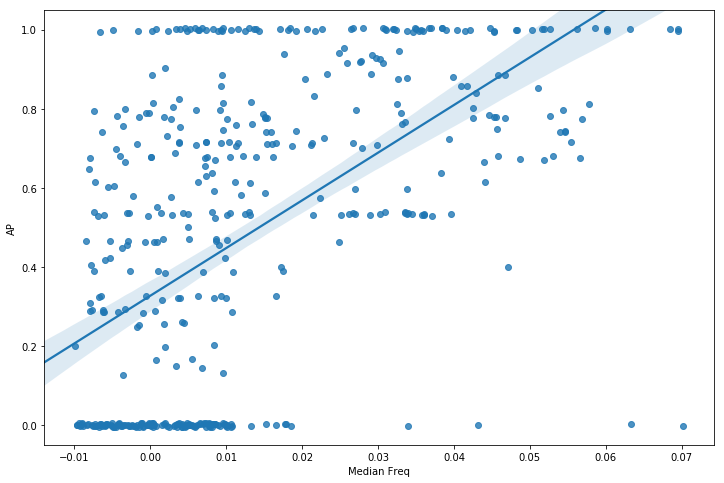
\includegraphics[width=0.5\textwidth]{images/scatter_crim.png}}\qquad
    \subbottom[Yamane]{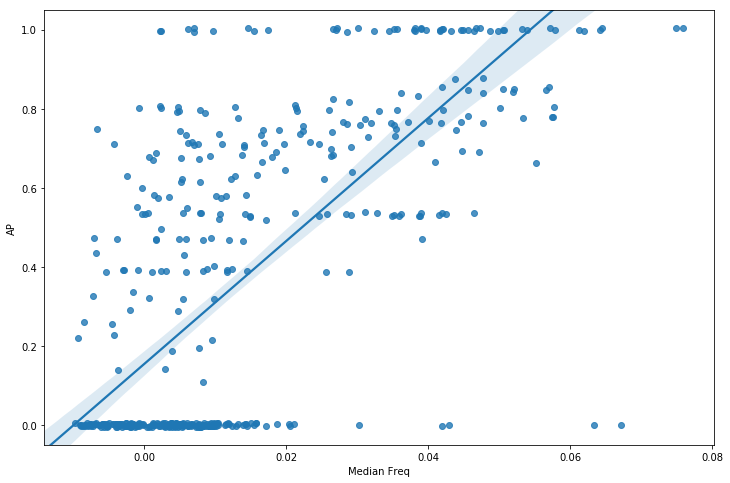
\includegraphics[width=0.5\textwidth]{images/scatter_yamane.png}}%
    \caption{Scatter-plot of median gold hypernym frequency against \ac{AP}.}        
    \label{fig:scatter_crim_yamane}
\end{figure}

There is a linear, positively-correlated relationship between the median frequency of the gold hypernyms which also feature in the training set and the precision of predicted hypernyms.\footnote{Note that query terms (i.e. hyponyms) feature in either the training set or test set but never in both.}  A cluster of points at the bottom-left of the charts represent query words which scored 0 \ac{AP}.  The model struggled to generate correct hypernyms on account of the absence of these words in the training set.  CRIM (top) shows more of a tendency to score well on seldom seen hypernyms, as attested by a larger concentration of point to the top-left of the plot than can be found in the same region of the Yamane plot.  The regression lines explain 0.31 and 0.51 of CRIM's and Yamane's hypernym frequency/score relationship respectively.  The median gold hypernym frequency has less predictive power in CRIM than in Yamane.  This might suggest that CRIM generalises more than Yamane, possibly due to the fact that gradient updates are computed on batches of 352 samples compared to just 6 samples in the case of Yamane.

Next, we investigated the negative hypernyms most often predicted with the highest confidence by each respective model, for query terms that yielded an \ac{AP} score of 0.  We plotted the 15 most common top-ranked, false positive words predicted by CRIM and Yamane respectively with histograms shown in Figure~\ref{fig:false_positive_crim_yamane}.
\begin{figure}[!ht]
    \centering
    \subbottom[CRIM]{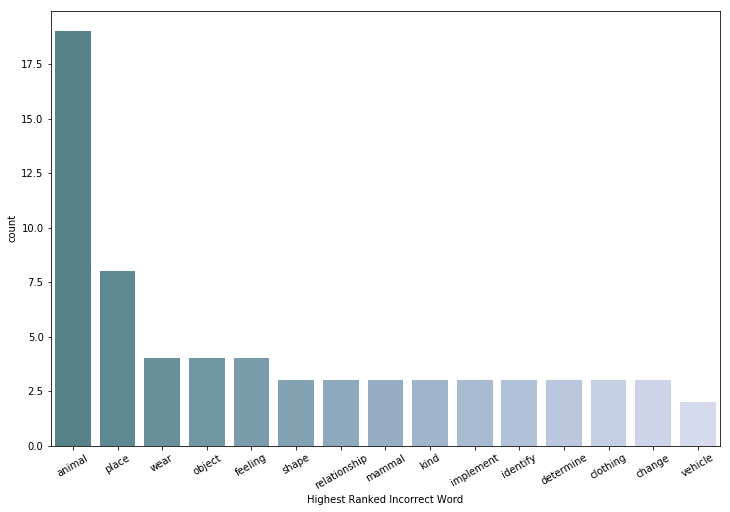
\includegraphics[width=0.6\textwidth]{images/crim_highest_ranked_incorrect.png}}\qquad
    \subbottom[Yamane]{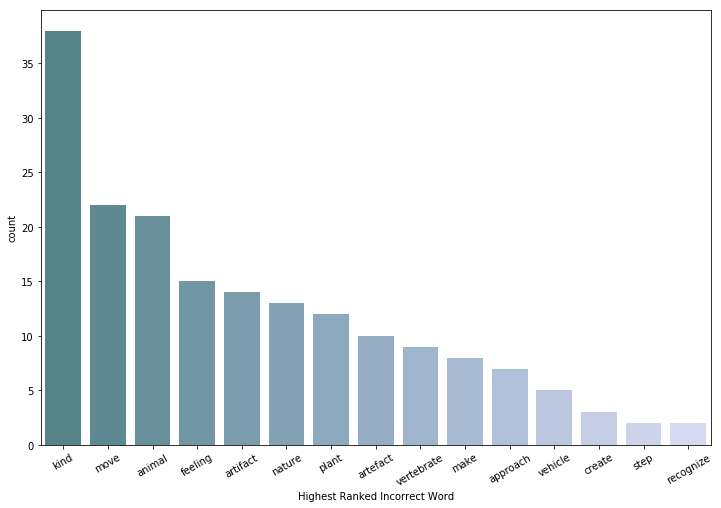
\includegraphics[width=0.6\textwidth]{images/yamane_highest_ranked_incorrect.png}}%
    \caption{Highest-ranked false positive hypernyms.}        
    \label{fig:false_positive_crim_yamane}
\end{figure}
Both CRIM and Yamane display a tendency to generate hypernyms which were often encountered during training such as \textit{animal}, \textit{plant} and \textit{object}.  Out of the 15 false positives most-commonly predicted by CRIM, two featured in the top ten highest occurring hypernyms in the training set. In the case of Yamane, five of these words were also on the top ten hypernym list.  Therefore, a shade of lexical memorisation can also be observed in projection learning models.  Perhaps, this phenomenon cannot be entirely avoided in the context of supervised learning.  

To restore some of our confidence in the capabilities of projection learning models, let us consider examples of terms which scored a perfect 1 \ac{AP}.  Moreover, we will only regard terms with hypernyms which seldom occur in the training set.  We will focus on CRIM, which has shown more ability to discover relatively rare hypernyms.  We reiterate that the length of the gold-standard list exerts a heavy weight on the scoring function we borrowed from the SemEval shared task \citep{camacho2018semeval}.  

\begin{table*}\centering
    \begin{tabular}{@{}lrrl@{}} \toprule
    \multicolumn{4}{c}{\textbf{CRIM Predictions}} \\
    \textit{Word} & \textit{AP} & \textit{Median Frequency} & \multicolumn{1}{c}{\textit{Top 5 Predictions}} \\ \midrule
    airship & 1. & 0.00373 & \textbf{vehicle}, \textbf{craft}, \textbf{aircraft}, airplane, artifact \\
    canoe & 1. & 0.00339 & \textbf{vehicle}, \textbf{boat}, \textbf{craft}, \textbf{vessel}, watercraft \\
    drape & 1. & 0.00271 & \textbf{cover}, wear, buy, sell, protect \\
    fog & 1. & 0.00085 & \textbf{weather}, change, place, shape, supply\\
    liberty & 1. & 0.00017 & \textbf{freedom}, liberty, belief, element, object\\
    square & 1. & 0.00119 & \textbf{shape}, place, form, figure, point\\
    violence & 1. & 0.00271 & \textbf{action}, violence, emotion, crime, anger\\
    yellow & 1. & 0.00237 & \textbf{color}, plant, crop, flower, green\\
    \bottomrule
    \end{tabular}
    \caption{Terms having low-frequency hypernyms correctly predicted by CRIM.}\label{tab:crim_perfect_score}
\end{table*}

Table~\ref{tab:crim_perfect_score} shows the top five hypernyms, predicted by CRIM \footnote{unregularised; 10 projections; 10 negative samples; trained on fastText word features for 15 epochs.}, for the terms having the least frequently occurring gold hypernyms.  Words in bold are gold-standard hypernyms and most terms in the table featured only a single gold-standard hypernym.  The model was unregularised, which explains why predictions at times include the term word itself (\textit{liberty}, \textit{violence}), or synonyms of the word (\textit{yellow}).  However, the model also surprises us with hypernyms which, despite being technically incorrect, are arguably precise.  Examples include, \textit{canoe} $\Rightarrow$ \textit{watercraft}; \textit{liberty} $\Rightarrow$ \textit{belief}; \textit{square} $\Rightarrow$ \textit{place}, \textit{form}, \textit{figure}; and \textit{violence} $\Rightarrow$ \textit{crime}. 

\subsection{Observations}

% CRIM is at least as good as Yamane
% Yamane's assertion that "joint learning" method is better "pipeline" model as he calls clustering together with piece-wise transformation matrix learning
% Choice of embeddings makes a real difference
% Increasing projections works, just on word2vec which is what bernier observed after running ablation tests
% during the shared task result evaluation
All configurations - irrespective of model, embeddings choice, clusters or regularisation comfortably beat the basic Cosine similarity and \ac{MFH} na\"ive baselines.  We did not evaluate these results statistically, since the improvement is obvious: for instance the fastText, single-cluster asymmetric model minimising \ac{MSE} beats the \ac{MFH} baseline by a 69\% margin.

With respect to the \ac{MSE} model family, there is strong empirical evidence which suggests that - on our chosen combined dataset and metrics - training a single-cluster, baseline model on fastText is the way to go.  We challenged the \citet{ustalov2017negative} assertion that regularisation has an effect on \ac{MSE} model performance.  Indeed, we found that regularisation has no significant effect on $M_1$ both in interaction with other factors, and in isolation.  This applied on all embeddings, including the same word2vec embeddings \citeauthor{ustalov2017negative} used in their English experiments.  However, we did not run an exhaustive grid-search tests to tune the $\lambda$ regularisation weighting parameter; instead we fixed the setting to 1, which was their chosen regularisation weight for re-projected regularisation.

\citet{Fu2014} findings were re-confirmed, despite the setup was modified in several ways: we recast their original problem as hypernym discovery; we evaluated on information retrieval metrics; we cross-validated the models on a different dataset.  Cluster size was certainly found to improve performance on word2vec embeddings, although the same did not hold for the other embeddings vector spaces, particulary fastText.

Introducing the regularisation terms proposed by \citet{ustalov2017negative} to a binary cross-entropy model (CRIM) did not really work out.  The effect was moderately negative, insofar that a significant result was only observed in one model setup out of 27.  Regularisation was not found to have any significant effect on \ac{MSE} models either.  

Increasing the projections in CRIM, had an adverse reaction when training the model on word2vec features.  \citet{bernier2018crim} reported a different empirical experience whereby multiple projections improved their \ac{MAP}/\ac{MRR} score.  This could be due to the interaction of the projection layer setting with one or several other setting.  The authors themselves specifically point out that they did not perform an in-depth analysis of their hyperparameter settings.  Moreover, they tune embeddings jointly with the projection matrices while decreasing the learning rate by a full order of magnitiude and training for several hundred epochs.  

In both \ac{MSE} and binary cross-entropy model types, fastText was proven to be the superior embeddings out of the three tested.  We believe this is a small contribution we made to the research area since, to our knowledge, projection learning models have so far only been evaluated on word2vec embeddings features.  Yamane, on the other hand, narrowed the gap between word2vec and fastText we had so far observed.  Yamane and CRIM were found to perform significantly better than \ac{MSE} models which \citet{yamane2016distributional} refer to as \say{pipeline models}. In this paper, the authors reported the superior performance of the "inner product" method, an assertion we found to be statistically sound.

The poor performance of GloVe, is probably due to how the embeddings training algorithm makes use of the dot product operator.  In word2vec and fastText, dot-product is used to estimate the similarity of the context word and target word (and vice versa depending on the model choice).  In GloVe the objective function encourages the dot product of word vectors to approximate the log of the co-occurrence probability of the words which may make the embeddings less suitable for our model.

